\documentclass[12pt]{article}
\usepackage{ctex}
\usepackage{amsthm,amsmath,amssymb}
\usepackage{amsfonts}
\usepackage{mathrsfs}
\usepackage{listings}
\usepackage{verbatim}
\usepackage{fancyhdr}
\usepackage{graphicx}
\usepackage{xeCJK}
\usepackage{xcolor}      %代码着色宏包
\usepackage{CJK}         %显示中文宏包
\usepackage{fontspec}
\usepackage{float}
\usepackage{placeins}
\usepackage{subfigure}
\usepackage{bm}
\usepackage{enumitem}
\usepackage[colorlinks,linkcolor=blue]{hyperref}

\lstset{
    basicstyle=\fontspec{Consolas},
    %numbers=left,
    %rulesepcolor=\color{red!20!green!20!blue!20},
    escapeinside=``,
    xleftmargin=2em,xrightmargin=2em, aboveskip=1em,
    %背景框
    framexleftmargin=1.5mm,
    frame=shadowbox,
    %背景色
    backgroundcolor=\color[RGB]{245,245,244},
    %样式
    keywordstyle=\color{blue}\fontspec{Consolas Bold},
    %identifierstyle=\bf,
	breaklines=true,
    numberstyle=\color[RGB]{0,192,192},
    commentstyle=\color[RGB]{96,96,96}\fontspec{Consolas Italic},
    stringstyle=\rmfamily\slshape\color[RGB]{128,0,0},
    %显示空格
    showstringspaces=false
}

\textheight 23cm \textwidth 15cm
\topmargin -1.5cm \oddsidemargin 0.3cm \evensidemargin -0.3cm

\begin{document}
\title {HW2-CAGD}
\date{\today}
\author{阚皓玮}
\maketitle
\section{使用说明}
在matlab中运行Hw2.m脚本文件,出现交互图窗。工具栏中点击红色按钮添加点,蓝色按钮De Casteljau算法得到Bézier曲线,绿色按钮Bernstein基表示得到Bézier曲线。

\section{实验内容}
\noindent 实现基于
\begin{enumerate}[itemsep= -6 pt,topsep = 0 pt]
    \item De Casteljau 递归算法
    \item Bernstein 基函数的代数方法
\end{enumerate}
的Bézier曲线生成,并且实现通过控制多边形获得 Bézier 曲线的交互式编辑功能。

\section{算法介绍}
 {\bf Input:}  控制多边形的点$\{b_0,b_1,...b_n\}$

{\bf Output:} Bézier曲线$x(t)$,其中$t\in[0,1]$

\noindent 下面介绍两种获得Bézier曲线的算法:

{\noindent\large \bf De Casteljau递归算法}

对于$t\in[0,1]$,我们按照如下步骤计算$x(t)$
\begin{enumerate}[itemsep= -6 pt,topsep = 0 pt]
    \item 将控制多边形的边每一条边按照t:(1-t)的比例分割得到相应的点
    \item 将新的点用按顺序用线连接
    \item 再次将新得到的线按1中比例连接分割得到新的点,并将新的点按顺序连接
    \item 按照3中方式重复以上步骤,直到只剩下一个点,即为$x(t)$
\end{enumerate}
{\noindent\large \bf 基于Bernstein基函数的代数表示方法}

基于Bernstein基函数,我们可将$x(t)$按如下方式表示
$$
    \displaystyle x(t)=\sum_{i=0}^nB_n^i(t)b_i
$$
其中$B_n^i(t)=\dbinom{n}{i}t^i(1-t)^{n-i}$

\section{实验结果}
实验交互选点得到Bézier曲线结果如下:
\begin{figure}[htb]
    \subfigure[De Casteljau]{
        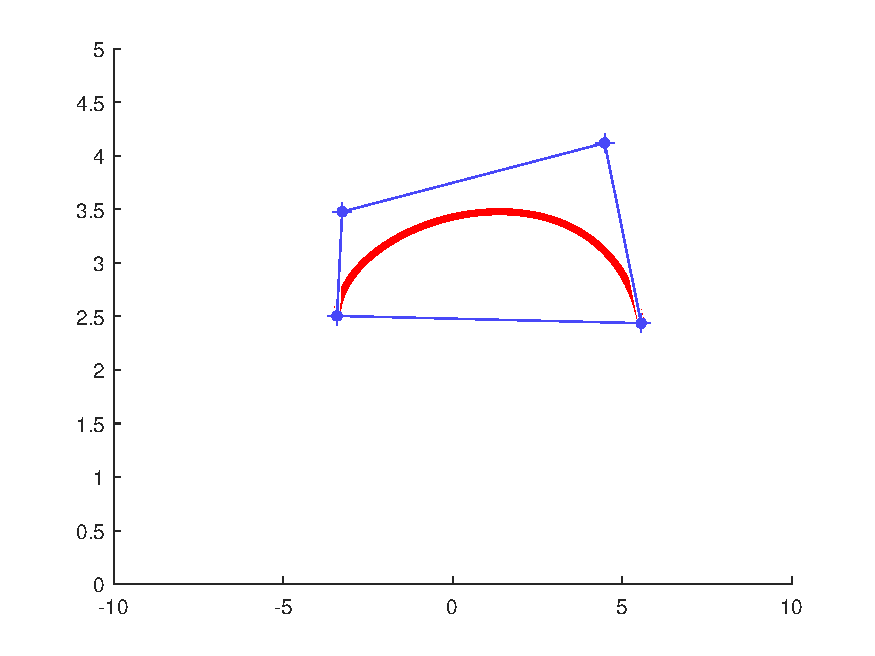
\includegraphics[width=0.5\textwidth]{result/d1.pdf}
    }
    \subfigure[Bernstein]{
        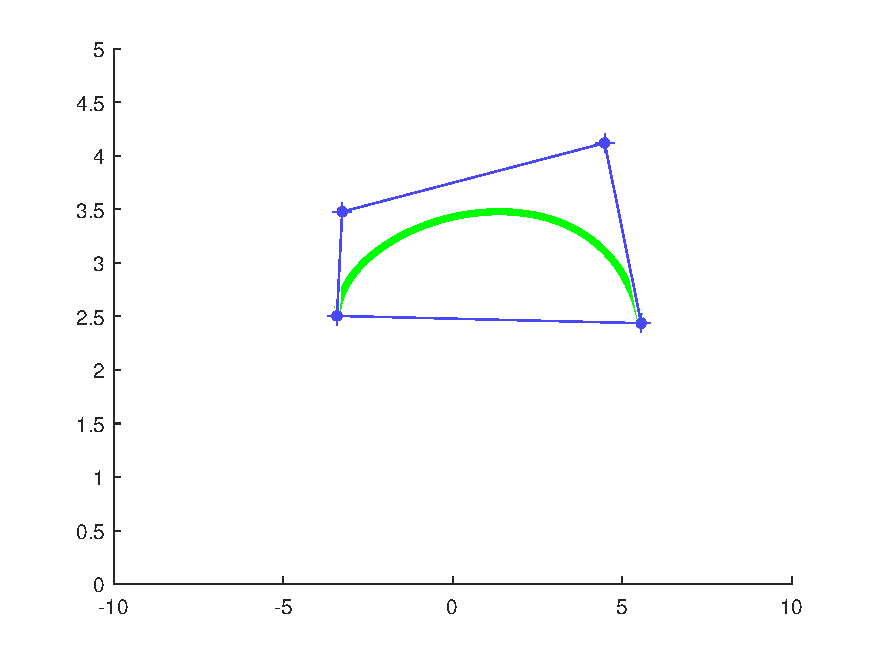
\includegraphics[width=0.5\textwidth]{result/b1.pdf}
    }
    \subfigure[De Casteljau]{
        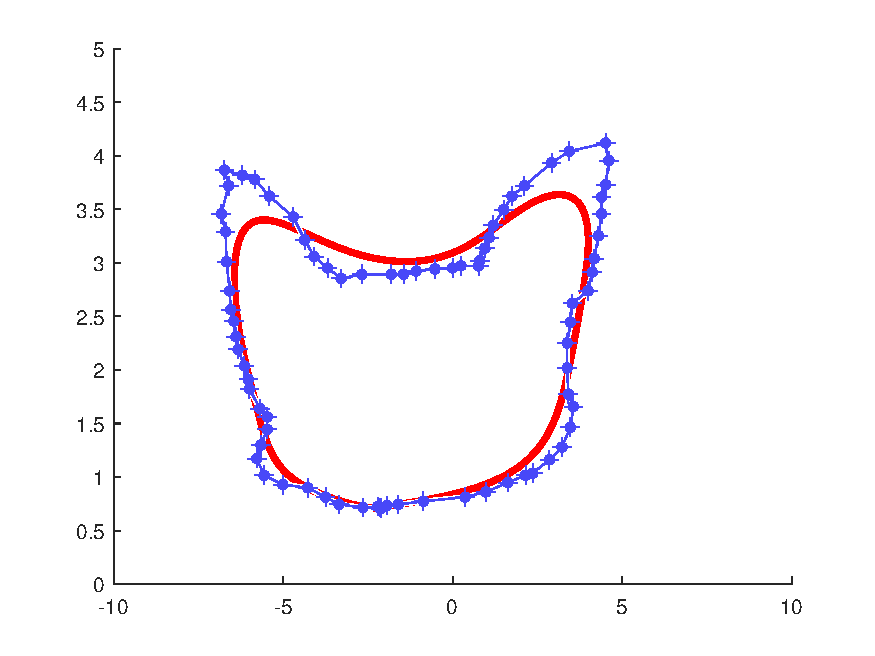
\includegraphics[width=0.5\textwidth]{result/d3.pdf}
    }
    \subfigure[Bernstein]{
        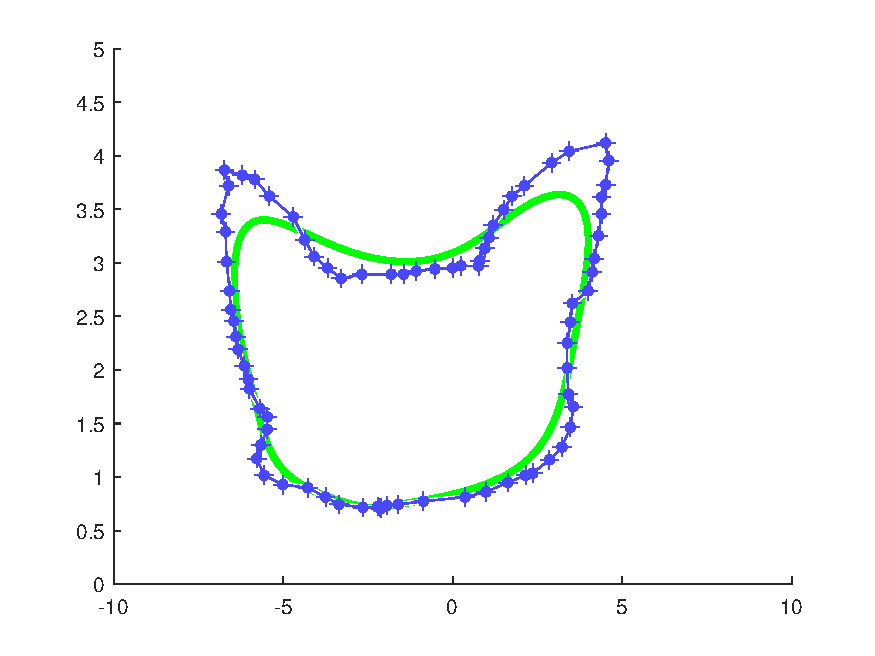
\includegraphics[width=0.5\textwidth]{result/b3.pdf}
    }
\end{figure}

\section{结果分析及比较}
两种算法获得的曲线是相同的,理论上Bernstein基函数的表示方法更易于表示且复杂度更低,但是实际实验过程中De Casteljau算法的效率更高,这可能是由于matlab中计算Bernstein函数的速度较慢。另一个基于Bernstein基函数的表示方法的缺点是,当控制点的数量较大时,Bernstein基函数中组合数的值较小,可能会超出计算机的精度范围,造成结果的不准确。因此在实际应用过程中,De Casteljau算法可能会是更好的选择

\appendix
\section{Code}
完整代码可从\url{https://github.com/mathendy/MS-USTC/tree/master/2020fall/CAGD/Hw2}下载

\end{document}